\section{The Map}\label{sec:social-combat-map}
\vfil

Social combat takes place on a zone map much as it does with personal combat. Instead of representing some physical geography, the map represents the social space of the encounter. Because of the kinds of options available to characters involved in social combat, certain kinds of map shapes have certain kinds of effects on behaviour and can be used to represent specific issues.

In general, concentric circles imply intimacy. Zone shapes with many borders, and therefore many avenues of escape and access, better represent socially open places like chatting about the weather at a party. Intimate zones are often objectives, such as when you want to get someone to reveal valuable information, and so you want to maneuver them into intimate, trusting conversation.

To begin with, moving between zones has no additional cost --- there is no initial use of ``borders'' as there is in personal combat. Characters in the same zone can be said to be engaging each other socially: they are conversing about interesting, relevant things that they care about. Conversely, the further apart characters are on the map, the more social distance is in their conversation. Range has a deep impact on the effectiveness of characters' interactions and so one must usually close the range before one can do anything useful, such as move the conversation to a more intimate space.

Zones represent in the first instance a degree of intimacy in the social context. This will sometimes correspond to a spatial dimension too, but more often it represents something much more nebulous. For instance, a separate zone might correspond to a small balcony where a conversation might occur. It is often a good idea for the table to design the map of the social combat as a group.

Optionally, once the map is created, each player may choose to place one free-taggable \Aspect{} on a single zone, or a pass value of 2 on a single border, to reflect the personal contours of the social situation.

% badbox here
% \newpage

\subsection{Time}\label{sec:Time}

For each zone on the map, create one time box to represent available time to resolve. If you need to know exactly how long something took, the table should determine the maximum amount of time something is allowed (even the best party will disperse by morning). If a victory condition is achieved before the time boxes run out, the maximum time can be downgraded a number of shifts on the Time Track (Dealing With Time, Chapter 2) equal to the number of unchecked boxes. Often, table consensus will determine a very similar result in any case.

\subsection{The Actors}\label{sec:The Actors}

One of the biggest conceptual hurdles in adopting this system for resolving social interactions is recognizing that not every person in a scene needs to be represented on the map. Part of this is embodied within the zones themselves, as \Aspects{} on the zones can represent the other people involved.

This can in fact be made even more abstract, when you want to make a situation tactical that has become mired or unproductive in regular role-play. By making some of the actors on the map ideas instead of explicit people, you can conduct a scientific investigation or any other information-revealing multi-step endeavour. Make the opposition the Fact and, maybe, an Attractive Falsehood and you can do science. Add in people with conflicting goals (a young whipper-snapper who wants to be primary author on the publication of your discovery!) and the abstract can engage the concrete in both directions.

\subsection{Victory}\label{sec:Victory}

Victory conditions should relate to map position. Usually the objective will be to get a certain person or persons into a specific zone before the timer runs out. This can be more complex, however, to achieve different goals: if you want to model persuading a crowd, you could score participants by how many crowd members are in their target zone when the timer runs out. Feel free to push the system around and find other victory conditions.

\subsection{Sample Maps}\label{sec:Sample Maps}

\subsubsection{Party}

A party has a lot of accessible conversation space --- everyone is there to chit-chat after all --- and probably at least one intimate space. It is well represented by a central shape with several attached shapes. Inside one attached space, add a couple of concentric circles for intimacy. An objective in the party might be to hook up with a powerful businessman and get him to brag about his company's secret operation on the dark side of the moon: you win if you can get him, yourself, and the science officer into the center of the intimate zone before the timer runs out.

The party map doesn't need to be complicated --- the simpler it is the faster things will go. The important thing is to make it take a few steps to get to the target zone and be complex enough to imply story with every move. The map above is about the minimum complexity you would want from a social combat map. It might be close to the maximum also!

\subsubsection{Seduction}

\begin{figure}
\centering\footnotesize
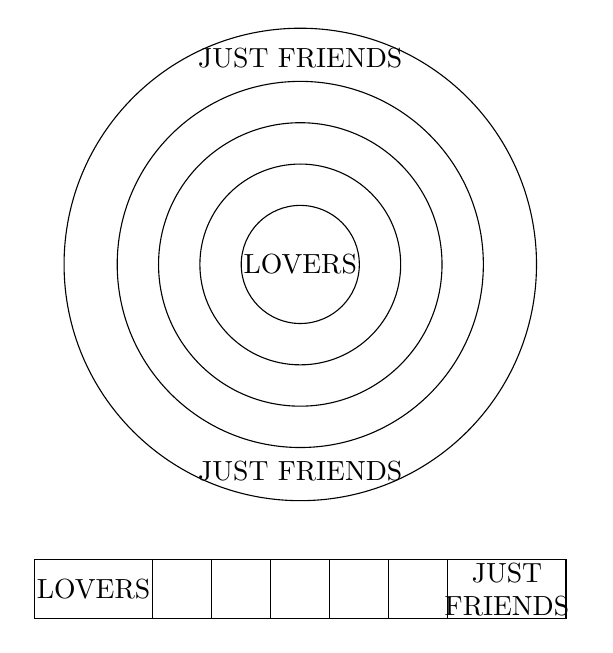
\begin{tikzpicture}[scale=0.75]
\begin{scope}
\draw circle (1) circle (1.7) circle (2.4) circle (3.1) circle (4.0)
  (0,0) node {LOVERS}
  (0,3.5) node {JUST FRIENDS}
  (0,-3.5) node {JUST FRIENDS};
\end{scope}
\begin{scope}[yshift=-5cm]
\draw
  (-2.5,0) rectangle +(-2,-1)
    +(-1,-0.5) node [anchor=center] {LOVERS}
  (2.5,0) rectangle +(2,-1)
    +(1,-0.5) node [text width=1.75cm,text centered] { JUST FRIENDS}
  \foreach \x in {-2.5,...,1.5} {
    (\x,0) rectangle ++(1,-1)
  }
;
\end{scope}
\end{tikzpicture}

\caption{Two sample social combat maps: Seduction}
\label{fig:social-combat-map-seduction}
\end{figure}


A seduction might be well modeled with a deep set of concentric circles --- say five or six --- with the objective of getting both characters in the bull's-eye. Such an engagement could have multiple suitors and possibly require removing some or all from the map through Composure damage.

Suitors might be PCs or they might be NPCs or in some cases they might just be ``pawns'' --- if there is a concept you want to be relevant to the goal but that doesn't necessarily need to have free will in the fight, just give it a marker and no statistics. Players can move it around towards or away from goals (voters in an election or observers at a debate!) but it doesn't do anything on its own.

This could also be done with a simple linear track of, say, seven zones. Mark the first zone \LOVERS{} and the last zone \JUSTFRIENDS{}. Start the seducer on or near \LOVERS{} and the objective on or near \JUSTFRIENDS{}. Start other competitive suitors anywhere that seems fun or scary.

If the objective and anyone else are together on the \LOVERS{} zone, it has fallen for that suitor. If the objective and anyone else are together on the \JUSTFRIENDS{} zone, whoever has joined the objective there is removed from play.

\subsubsection{Debate}

\begin{figure}
\centering\footnotesize
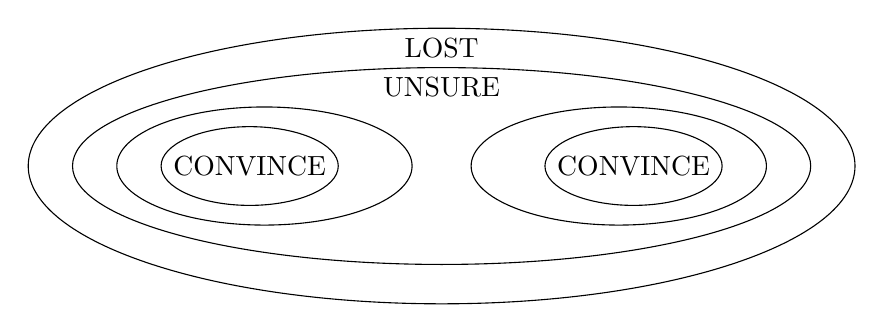
\begin{tikzpicture}[xscale=0.75,yscale=0.5]
\begin{scope}
\draw
  (-3,0) circle (2.5 and 1.5)
  (-3.25,0)   circle (1.5 and 1) node {CONVINCE}
  (0,0) ellipse (7 and 3.5) (0,3) node {LOST}
  (0,0) ellipse (6.25 and 2.5) (0,2) node {UNSURE}
  (3,0) circle (2.5 and 1.5)
  (3.25,0)   circle (1.5 and 1) node {CONVINCE}
%   (-3,0) node {CONVINCE}
%   (0,3.5) node {JUST FRIENDS}
%   (0,-3.5) node {JUST FRIENDS}
;
\end{scope}
% \begin{scope}[yshift=-5cm]
% \draw
%   (-2.5,0) rectangle +(-2,-1)
%     +(-1,-0.5) node [anchor=center] {LOVERS}
%   (2.5,0) rectangle +(2,-1)
%     +(1,-0.5) node [text width=1.75cm,text centered] { JUST FRIENDS}
%   \foreach \x in {-2.5,...,1.5} {
%     (\x,0) rectangle ++(1,-1)
%   }
% ;
% \end{scope}
\end{tikzpicture}

\caption{Sample social combat map: Debate}
\label{fig:social-combat-map-debate}
\end{figure}

A debate can be modeled with two sets of concentric circles representing opposing perspectives. The objective would be to move the opponent into your own central circle or moving the majority of audience members into your zone. Note that because of the steep drop-off in effectiveness at range, it will be necessary to move towards your opponent in order to engage him and pull him back to see your point (answering his specific arguments, showing sympathy and understanding).

